\section{Example}

In this chapter both approaches should be demonstrated within the example of a movie management software.  

\subsection{Automatic Test Generation: A Use Case Driven Approach}

In the first step the test objectives have to be derived. Therefore we define the use cases and their contracts as requirement-level logical expressions. Only the use cases that really impact the state of the transition system were specified for this example. The notation used is equal to the one proposed in the paper. 

\begin{lstlisting}
UC createMovie(m: movie)
post createdMovie(m)

UC createLinkedPerformer(p: performer, m: movie)
pre createdMovie(m)
post createdPerformer(p) and createdLink(p,m)

UC rateMovie(m: movie)
pre createdMovie(m)
post calculatedOverallRating(m)

UC ratePerformer(p: performer)
pre createdPerformer(p)
post forall(m: movie){ createdLink(p,m)@pre implies calculatedOverallRating(m) }

UC linkExistingMovie(m: movie, p: performer)
pre createdMovie(m) and createdPerformer(p)
post not createdLink(p,m)@pre implies (createdLink(p,m) and calculatedOverallRating(m))

UC linkExistingPerformer(m: movie, p: performer)
pre createdMovie(m) and createdPerformer(p)
post not createdLink(p,m)@pre implies (createdLink(p,m) and calculatedOverallRating(m))

UC unlinkMovie(m: movie, p: performer)
pre createdMovie(m) and createdPerformer(p) and createdLink(p,m)
post calculatedOverallRating(m) and not createdLink(p,m) and not exists(m2: movie){ createdLink(p,m2) }@pre implies not createdPerformer(p)

UC unlinkPerformer(m: movie, p: performer)
pre createdMovie(m) and createdPerformer(p) and createdLink(p,m)
post calculatedOverallRating(m) and not createdLink(p,m) and not exists(m2: movie){ createdLink(p,m2) }@pre implies not createdPerformer(p)

UC removeMovie(m: movie)
pre createdMovie(m)
post not createdMovie(m) and forall(p: performer){ not createdLink(p,m) } and not exist(m2: movie){ createdLink(p,m2) }@pre implies not createdPerformer(p)

UC removePerformer(p: performer)
pre createdPerformer(p)
post not createdPerformer(p) and forall(m: movie){ not createdLink(p,m) }
\end{lstlisting}

After that the UCSystem tool should build the UCTS (\autoref{ucts}) through exhaustive simulation. The pool of parameters was restricted to one movie and performer to avoid a combinatorical explosion for this example. Furthermore the predicate calculatedOverallRating is no longer considered. Note that only predicates that evaluate to true are listed in the states as in the original paper. 

\begin{figure}[h]
	\centering
	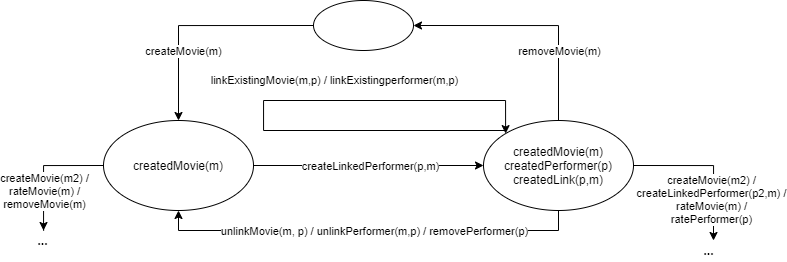
\includegraphics[width=1.0\textwidth]{img/ucts.png}
	\label{ucts}
\end{figure}

Depending on the selected coverage criterion, we receive different test objectives. How many test objectives are derived depends on the internal implementation of UCSystem and cannot be predicted for this example. Let's assume that one test objective is the test path createMovie(m) -> createLinkedPerformer(p,m) -> removeMovie(m). Then the use case scenarios from \autoref{ucs} are used to replace the use cases in the test objectives. 

\begin{figure}[h]
	\centering
	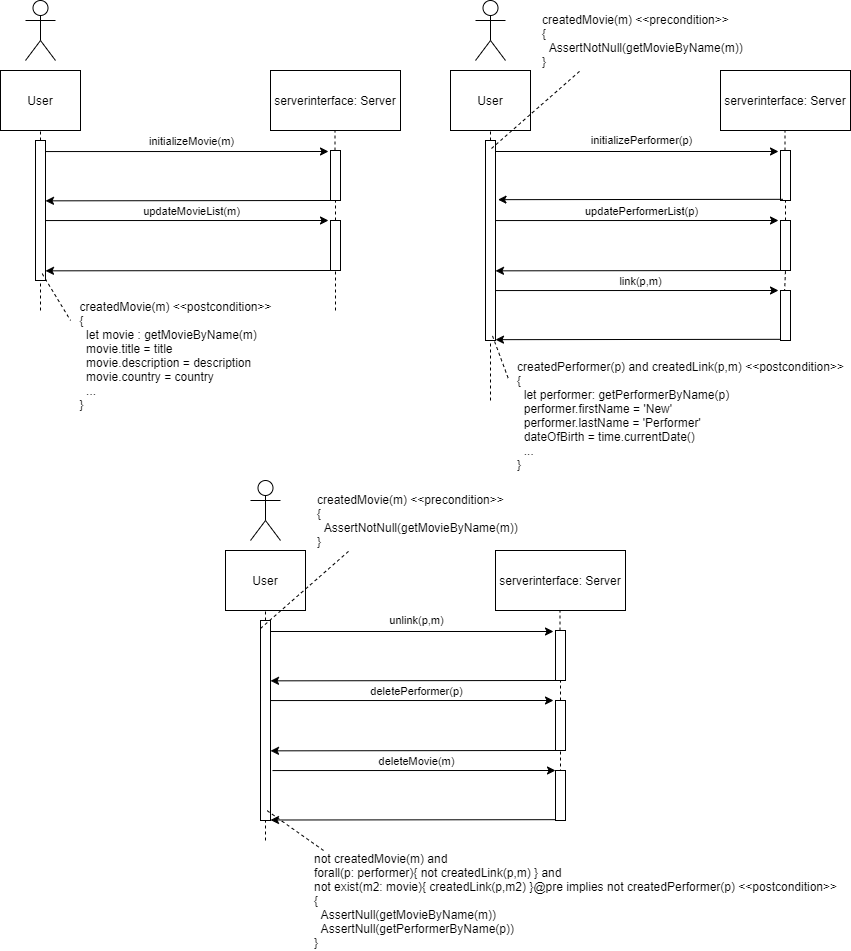
\includegraphics[width=0.65\textwidth]{img/ucs.png}
	\label{ucs}
\end{figure}

The UC-SCSystem uses the shown implementation in the use case scenarios to derive executable test scenarios. 

\subsection{An Automated Approach to System Testing based on Scenarios and Operations Contracts}

Input to the approach in this paper is the IOD (\autoref{iod}) with separate contracts defined in an OCL file. 

\begin{figure}[h]
	\centering
	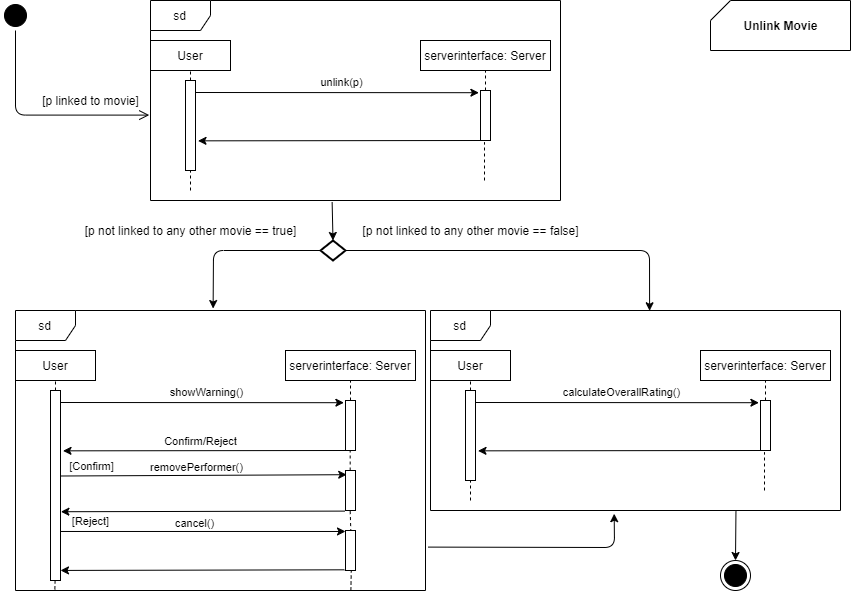
\includegraphics[width=0.65\textwidth]{img/iod.png}
	\label{iod}
\end{figure}

\begin{lstlisting}
context Movie::unlink(performer)
pre  self.performers[performer] -> not isEmpty()
post self.performers[performer] -> isEmpty()

context MovieManager::removePerformer(performer)
pre forAll(movie | movie.performers[performer] -> isEmpty())
post self.performers[performer] -> isEmpty()

context Movie::calculateOverallRating()
post self.rating = 0.5 * (self.mean(self.performers.getRatings()) + self.rating)
\end{lstlisting}

Then the CTS matrix gets defined:

\begin{longtable}[h]{p{0.5cm}p{0.5\textwidth}p{0.5\textwidth}}
	Nr. & Approach \cite{ansatz.2006} & Approach \cite{ansatz.2007} \\
	3a & 
	Use cases describing the basic operations in the transition system. Contracts that are attached to the use cases describing the states in the transition system. The transition system (UCTS) itself as a simulation model to derive test objectives from. Test objectives describing the test paths. UCSystem as a third party tool to build the UCTS and to derive test objectives using coverage criteria. Use case scenarios to build test scenarios from test objectives. UC-SCSystem to generate executable test scenarios.  & 
	IODs holding all scenarios and operations of a use case. Operations can either be interaction uses or sequence diagrams inside the IOD. Contracts written in OCL that are attached to the operations describing the states in the transition system. The CTS describing the transition system. Test paths derived from the CTS using coverage criteria.  \\
\end{longtable}